% A Stack-Based Bytecode Virtual Machine for the Lattice Programming Language
%
% Compile with: pdflatex lattice_vm.tex && pdflatex lattice_vm.tex
%
\documentclass[11pt]{article}

\usepackage[margin=1in]{geometry}
\usepackage{amsmath,amssymb,amsthm}
\usepackage{mathpartir}
\usepackage{stmaryrd}        % \llbracket, \rrbracket
\usepackage{xcolor}
\usepackage{microtype}
\usepackage{enumitem}
\usepackage{booktabs}
\usepackage{listings}
\usepackage{tikz}
\usepackage{pgfplots}
\usepackage{hyperref}
\usepackage{needspace}
\usepackage{float}
\usepackage{multirow}

\usetikzlibrary{shapes.geometric, arrows.meta, positioning, fit, backgrounds, calc, decorations.pathreplacing, patterns}
\pgfplotsset{compat=1.17}

% ── Theorem environments ──
\newtheorem{theorem}{Theorem}[section]
\newtheorem{lemma}[theorem]{Lemma}
\newtheorem{proposition}[theorem]{Proposition}
\newtheorem{corollary}[theorem]{Corollary}
\newtheorem{definition}[theorem]{Definition}
\newtheorem{remark}[theorem]{Remark}

% ── Notation macros (reused from companion papers) ──
\newcommand{\kw}[1]{\mathbf{#1}}
\newcommand{\flx}{\kw{flux}}
\newcommand{\fixkw}{\kw{fix}}
\newcommand{\letkw}{\kw{let}}
\newcommand{\freezekw}{\kw{freeze}}
\newcommand{\thawkw}{\kw{thaw}}
\newcommand{\clonekw}{\kw{clone}}
\newcommand{\returnkw}{\kw{return}}
\newcommand{\spawnkw}{\kw{spawn}}

% Phase tags
\newcommand{\fluid}{\mathsf{fluid}}
\newcommand{\crystal}{\mathsf{crystal}}
\newcommand{\unphased}{\bot}

% VM-specific notation
\newcommand{\opcode}[1]{\texttt{OP\_#1}}
\newcommand{\Stack}{\mathsf{Stack}}
\newcommand{\Frames}{\mathsf{Frames}}
\newcommand{\Globals}{\mathsf{Globals}}
\newcommand{\Upvals}{\mathsf{Upvals}}
\newcommand{\promote}{\mathsf{promote}}
\newcommand{\rnone}{\mathsf{REGION\_NONE}}
\newcommand{\reph}{\mathsf{REGION\_EPHEMERAL}}

% ── Listings configuration ──
\lstdefinelanguage{Lattice}{
  morekeywords={fn,let,flux,fix,struct,if,else,for,in,while,return,freeze,thaw,clone,forge,true,false,print,spawn,scope,select,match,try,catch,throw,defer,import,enum,break,continue,loop,test,ensure,require},
  sensitive=true,
  morecomment=[l]{//},
  morecomment=[s]{/*}{*/},
  morestring=[b]",
  literate={->}{$\rightarrow$}{2},
}

\lstdefinestyle{clang}{
  language=C,
  basicstyle=\small\ttfamily,
  keywordstyle=\bfseries,
  commentstyle=\itshape\color{gray},
  stringstyle=\color{darkgray},
  numbers=left,
  numberstyle=\tiny\color{gray},
  numbersep=5pt,
  frame=single,
  framesep=3pt,
  xleftmargin=1.5em,
  breaklines=true,
  captionpos=b,
  aboveskip=0.8\baselineskip,
  belowskip=0.5\baselineskip,
  morekeywords={uint8_t,uint16_t,int64_t,size_t,bool,LatValue,Chunk,ObjUpvalue,CallFrame,VM,Env,Compiler,PhaseTag},
}

\lstset{
  language=Lattice,
  basicstyle=\small\ttfamily,
  keywordstyle=\bfseries,
  commentstyle=\itshape\color{gray},
  stringstyle=\color{darkgray},
  numbers=left,
  numberstyle=\tiny\color{gray},
  numbersep=5pt,
  frame=single,
  framesep=3pt,
  xleftmargin=1.5em,
  breaklines=true,
  captionpos=b,
  aboveskip=0.8\baselineskip,
  belowskip=0.5\baselineskip,
}

% ── Document ──
\title{\textbf{A Stack-Based Bytecode Virtual Machine\\for the Lattice Programming Language}}
\author{Alex Jokela\\{\small\texttt{alex.c.jokela@gmail.com}}}
\date{February 2026}

\begin{document}
\maketitle

\begin{abstract}
The Lattice language's original tree-walking interpreter incurred per-node
dispatch overhead and required AST retention for concurrency primitives.
We present a bytecode virtual machine that achieves full feature parity---including
the phase system, concurrent \texttt{scope}/\texttt{spawn}/\texttt{select},
exception handling, and modules---with significantly lower dispatch overhead.
Key contributions include: a 100-opcode instruction set with wide constant
variants and specialized integer fast paths, a single-pass compiler with
upvalue-based lexical closures, pre-compiled sub-chunks for concurrency
primitives that eliminate all runtime AST dependency, an ephemeral bump arena
for short-lived string temporaries, a binary serialization format
(\texttt{.latc}) for ahead-of-time distribution, and a self-hosted compiler
written in Lattice itself.  The implementation is validated by 815 tests
passing under AddressSanitizer with zero memory errors.
\end{abstract}

%% ─────────────────────────────────────────────────────────────────────────────
\section{Introduction}
\label{sec:intro}

The Lattice programming language~\cite{jokela2026lattice} introduces a
\emph{phase system} in which every runtime value carries a phase tag---either
$\fluid$ (mutable) or $\crystal$ (deeply immutable)---with explicit transitions
mediated by $\freezekw$, $\thawkw$, $\clonekw$, and $\kw{forge}$ operations.
The original implementation described in~\cite{jokela2026lattice} is a
tree-walking interpreter: the evaluator traverses AST nodes directly,
dispatching on each node's tag.  While straightforward, this approach has three
significant limitations.

\paragraph{Interpreter overhead.}
Each AST node visit incurs a switch dispatch, pointer chasing through the tree
structure, and recursive function call overhead.  For tight loops and
deeply nested expressions, these costs dominate execution time.

\paragraph{AST retention for concurrency.}
Lattice's structured concurrency primitives---\texttt{scope}, \texttt{spawn},
and \texttt{select}---require evaluating sub-expressions in spawned threads.
In the tree-walker, this means the AST must remain live for the duration of
concurrent execution, preventing the program representation from being
discarded after compilation.

\paragraph{Inability to serialize.}
A tree-walking interpreter ties execution to the AST, making it impossible
to compile a program once and distribute the compiled artifact.  Users must
ship source code and re-parse on every invocation.

This paper presents a bytecode virtual machine that addresses all three
limitations while maintaining full feature parity with the tree-walker.
The VM has been the default execution mode since Lattice v0.3.5; the
tree-walker remains available via the \texttt{-{}-tree-walk} flag.

\paragraph{Contributions.}
\begin{enumerate}[leftmargin=2em]
  \item A 100-opcode instruction set with variable-length encoding, wide
        constant variants for programs exceeding 256 constants, and
        specialized integer operations (\S\ref{sec:isa}).
  \item A single-pass bytecode compiler with upvalue-based closures,
        constant folding, and peephole optimizations (\S\ref{sec:compiler},
        \S\ref{sec:closures}).
  \item Pre-compiled sub-chunks for concurrency primitives, eliminating
        all runtime AST dependency (\S\ref{sec:concurrency}).
  \item A binary serialization format (\texttt{.latc}) enabling
        ahead-of-time compilation and distribution (\S\ref{sec:serialization}).
  \item A self-hosted compiler written in Lattice (\S\ref{sec:selfhost}).
  \item Empirical validation via 815 tests passing under both normal and
        AddressSanitizer builds (\S\ref{sec:eval}).
\end{enumerate}

%% ─────────────────────────────────────────────────────────────────────────────
\section{Instruction Set Architecture}
\label{sec:isa}

\subsection{Design Overview}

The Lattice VM uses a stack-based architecture with variable-length
instruction encoding.  Each instruction begins with a single-byte opcode
(values 0--99), optionally followed by one or more operand bytes.
The instruction set comprises 100 opcodes organized into 14 functional
categories (Table~\ref{tab:opcodes}).

We chose a stack-based design over a register-based design (as used by
Lua~5~\cite{ierusalimschy2005implementation}) for several reasons:
(1) simpler code generation---the compiler never needs to perform register
allocation; (2) more compact bytecode---stack instructions are typically
1--3 bytes versus 4 bytes for register triples; and (3) natural fit for
expression evaluation in a dynamically typed language where operand types
are not known at compile time.

\subsection{Opcode Categories}

\begin{table}[H]
\centering
\small
\caption{Instruction set overview (100 opcodes, indices 0--99).}
\label{tab:opcodes}
\begin{tabular}{@{}llr@{}}
\toprule
\textbf{Category} & \textbf{Representative opcodes} & \textbf{Count} \\
\midrule
Stack manipulation   & \opcode{CONSTANT}, \opcode{NIL}, \opcode{POP}, \opcode{DUP}, \opcode{SWAP}       & 8  \\
Arithmetic/logical   & \opcode{ADD}, \opcode{SUB}, \opcode{MUL}, \opcode{DIV}, \opcode{NEG}, \opcode{NOT} & 7  \\
Bitwise              & \opcode{BIT\_AND}, \opcode{BIT\_OR}, \opcode{LSHIFT}, \opcode{RSHIFT}             & 6  \\
Comparison           & \opcode{EQ}, \opcode{NEQ}, \opcode{LT}, \opcode{GT}, \opcode{LTEQ}, \opcode{GTEQ} & 6 \\
String               & \opcode{CONCAT}                                                                    & 1  \\
Variables            & \opcode{GET\_LOCAL}, \opcode{SET\_LOCAL}, \opcode{GET/SET\_GLOBAL}, \opcode{GET/SET\_UPVALUE} & 8 \\
Control flow         & \opcode{JUMP}, \opcode{JUMP\_IF\_FALSE}, \opcode{LOOP}                             & 5  \\
Functions            & \opcode{CALL}, \opcode{CLOSURE}, \opcode{RETURN}                                   & 3  \\
Iterators            & \opcode{ITER\_INIT}, \opcode{ITER\_NEXT}                                           & 2  \\
Data structures      & \opcode{BUILD\_ARRAY}, \opcode{INDEX}, \opcode{INVOKE}, \opcode{GET\_FIELD}        & 15 \\
Exceptions/defer     & \opcode{PUSH\_EXCEPTION\_HANDLER}, \opcode{THROW}, \opcode{DEFER\_PUSH}            & 6  \\
Phase system         & \opcode{FREEZE}, \opcode{THAW}, \opcode{REACT}, \opcode{BOND}, \opcode{SEED}       & 14 \\
Builtins/modules     & \opcode{PRINT}, \opcode{IMPORT}                                                    & 2  \\
Concurrency          & \opcode{SCOPE}, \opcode{SELECT}                                                    & 2  \\
Integer fast paths   & \opcode{INC\_LOCAL}, \opcode{ADD\_INT}, \opcode{LOAD\_INT8}                         & 8  \\
Wide variants        & \opcode{CONSTANT\_16}, \opcode{CLOSURE\_16}                                        & 5  \\
Special              & \opcode{RESET\_EPHEMERAL}, \opcode{HALT}                                           & 2  \\
\midrule
\textbf{Total}       &                                                                                    & \textbf{100} \\
\bottomrule
\end{tabular}
\end{table}

\subsection{Encoding Formats}

Instructions use four encoding formats, shown in Figure~\ref{fig:encoding}:

\begin{figure}[H]
\centering
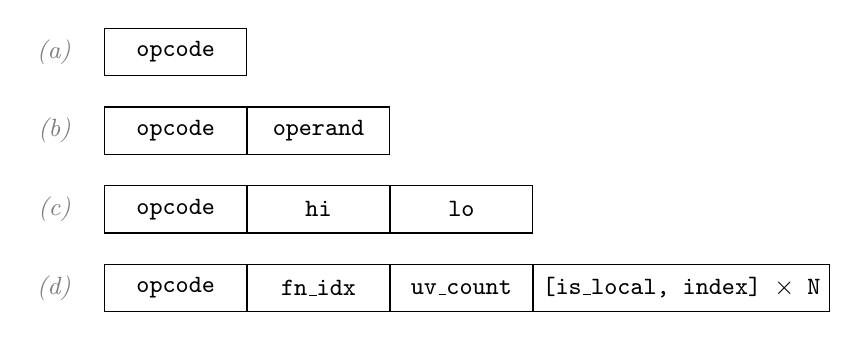
\begin{tikzpicture}[
  byte/.style={draw, minimum width=1.8cm, minimum height=0.6cm, font=\small\ttfamily},
  label/.style={font=\small\itshape, text=gray},
]
% Format 1: single byte
\node[byte] (op1) at (0,0) {opcode};
\node[label, left=0.3cm of op1] {(a)};

% Format 2: 1-operand
\node[byte] (op2) at (0,-1) {opcode};
\node[byte, right=0pt of op2] (arg2) {operand};
\node[label, left=0.3cm of op2] {(b)};

% Format 3: 2-byte operand (BE16)
\node[byte] (op3) at (0,-2) {opcode};
\node[byte, right=0pt of op3] (hi3) {hi};
\node[byte, right=0pt of hi3] (lo3) {lo};
\node[label, left=0.3cm of op3] {(c)};

% Format 4: variable-length (closure)
\node[byte] (op4) at (0,-3) {opcode};
\node[byte, right=0pt of op4] (idx4) {fn\_idx};
\node[byte, right=0pt of idx4] (cnt4) {uv\_count};
\node[byte, right=0pt of cnt4, minimum width=3.2cm] (uvs4) {[is\_local, index] $\times$ N};
\node[label, left=0.3cm of op4] {(d)};
\end{tikzpicture}
\caption{Instruction encoding formats: (a)~zero-operand, (b)~single-operand,
(c)~16-bit big-endian operand, (d)~variable-length (\opcode{CLOSURE}).}
\label{fig:encoding}
\end{figure}

\noindent
Most instructions use format~(a) or~(b).  Jump instructions use format~(c)
with a 16-bit signed offset.  The wide variants (\opcode{CONSTANT\_16},
\opcode{GET\_GLOBAL\_16}, etc.)\ also use format~(c), addressing up to 65,536
constants per chunk.  The \opcode{CLOSURE} and \opcode{SCOPE}/\opcode{SELECT}
instructions use format~(d) with variable-length trailing data.

\subsection{The Chunk Data Structure}

\needspace{12\baselineskip}
Each compiled function (or top-level script) is represented by a \texttt{Chunk}:

\begin{lstlisting}[style=clang,caption={The Chunk structure.}]
typedef struct {
    uint8_t  *code;         // bytecode stream
    size_t    code_len, code_cap;
    LatValue *constants;    // constant pool
    size_t    const_len, const_cap;
    int      *lines;        // source line per byte
    size_t    lines_len, lines_cap;
    char    **local_names;  // slot -> variable name
    size_t    local_name_cap;
    char     *name;         // function name (debug)
} Chunk;
\end{lstlisting}

The \texttt{constants} pool stores literal values (integers, floats, strings)
and, crucially, nested function chunks.  A compiled function is stored as a
\texttt{VAL\_CLOSURE} with \texttt{body\,=\,NULL} and
\texttt{native\_fn\,=\,Chunk*}, a convention we detail in
\S\ref{sec:closures}.  The \texttt{local\_names} array provides debug
information mapping stack slots to variable names, used both for error
reporting and for exporting locals to the environment during concurrent
execution (\S\ref{sec:concurrency}).

\subsection{Detailed Opcode Listing}

Table~\ref{tab:opcodes-full} provides a complete listing of all 100 opcodes
organized by category, with their numeric values and operand formats.

\begin{table}[H]
\centering
\small
\caption{Complete opcode listing with numeric values (0--99).}
\label{tab:opcodes-full}
\begin{tabular}{@{}rlll@{}}
\toprule
\textbf{Range} & \textbf{Category} & \textbf{Opcodes} & \textbf{Format} \\
\midrule
0--7   & Stack   & \texttt{CONSTANT}, \texttt{NIL}, \texttt{TRUE}, \texttt{FALSE}, \texttt{UNIT}, \texttt{POP}, \texttt{DUP}, \texttt{SWAP} & (a)/(b) \\
8--14  & Arith   & \texttt{ADD}, \texttt{SUB}, \texttt{MUL}, \texttt{DIV}, \texttt{MOD}, \texttt{NEG}, \texttt{NOT} & (a) \\
15--20 & Bitwise & \texttt{BIT\_AND/OR/XOR/NOT}, \texttt{LSHIFT}, \texttt{RSHIFT} & (a) \\
21--26 & Compare & \texttt{EQ}, \texttt{NEQ}, \texttt{LT}, \texttt{GT}, \texttt{LTEQ}, \texttt{GTEQ} & (a) \\
27     & String  & \texttt{CONCAT} & (a) \\
28--35 & Vars    & \texttt{GET/SET\_LOCAL}, \texttt{GET/SET/DEFINE\_GLOBAL}, \texttt{GET/SET\_UPVALUE}, \texttt{CLOSE\_UPVALUE} & (b) \\
36--40 & Jumps   & \texttt{JUMP}, \texttt{JUMP\_IF\_FALSE/TRUE/NOT\_NIL}, \texttt{LOOP} & (c) \\
41--43 & Funcs   & \texttt{CALL}, \texttt{CLOSURE}, \texttt{RETURN} & (b)/(d) \\
44--45 & Iter    & \texttt{ITER\_INIT}, \texttt{ITER\_NEXT} & (a)/(c) \\
46--60 & Data    & \texttt{BUILD\_*}, \texttt{INDEX}, \texttt{SET\_INDEX}, \texttt{GET/SET\_FIELD}, \texttt{INVOKE*} & (b)/multi \\
61--64 & Except  & \texttt{PUSH/POP\_EXCEPTION\_HANDLER}, \texttt{THROW}, \texttt{TRY\_UNWRAP} & (c)/(a) \\
65--66 & Defer   & \texttt{DEFER\_PUSH}, \texttt{DEFER\_RUN} & (c)/(a) \\
67--80 & Phase   & \texttt{FREEZE}, \texttt{THAW}, \texttt{CLONE}, \texttt{MARK\_FLUID}, \texttt{REACT}, etc. & (a)/multi \\
81--82 & Misc    & \texttt{PRINT}, \texttt{IMPORT} & (b) \\
83--84 & Concur  & \texttt{SCOPE}, \texttt{SELECT} & (d) \\
85--92 & IntOpt  & \texttt{INC/DEC\_LOCAL}, \texttt{ADD/SUB/MUL/LT/LTEQ\_INT}, \texttt{LOAD\_INT8} & (b)/(a) \\
93--97 & Wide    & \texttt{CONSTANT\_16}, \texttt{GET/SET/DEFINE\_GLOBAL\_16}, \texttt{CLOSURE\_16} & (c)/(d) \\
98--99 & Special & \texttt{RESET\_EPHEMERAL}, \texttt{HALT} & (a) \\
\bottomrule
\end{tabular}
\end{table}

Several design choices merit discussion.  The integer fast-path opcodes
(85--92) bypass the type-checking overhead of their generic counterparts:
\opcode{ADD\_INT} assumes both operands are \texttt{VAL\_INT} and produces
an \texttt{int64\_t} result directly, while the generic \opcode{ADD} must
check for string concatenation, float promotion, and type errors.  The
\opcode{LOAD\_INT8} instruction encodes a signed byte directly in the
instruction stream, avoiding constant pool allocation for the most common
small integer values.

The phase system opcodes (67--80) include both simple operations
(\opcode{FREEZE}, \opcode{THAW}, \opcode{CLONE}) that operate on the top
of stack, and variable-targeted operations (\opcode{FREEZE\_VAR},
\opcode{THAW\_VAR}, \opcode{SUBLIMATE\_VAR}) that take a variable name
index and location descriptor.  The latter enable the compiler to emit
\opcode{DUP} + \opcode{SET} write-back sequences when \texttt{freeze(x)} or
\texttt{thaw(x)} is called with an identifier argument, ensuring the
variable itself is updated rather than just the stack copy.

%% ─────────────────────────────────────────────────────────────────────────────
\section{The Bytecode Compiler}
\label{sec:compiler}

\subsection{Architecture}

The compiler performs a single-pass walk over the AST produced by the parser.
It maintains a chain of \texttt{Compiler} structs linked via \texttt{enclosing}
pointers, one per lexical scope that introduces a new function:

\begin{lstlisting}[style=clang,caption={The Compiler structure (simplified).}]
typedef struct Compiler {
    struct Compiler *enclosing;
    Chunk       *chunk;
    FunctionType type;     // SCRIPT, FUNCTION, CLOSURE
    char        *func_name;
    int          arity;
    Local       *locals;
    size_t       local_count, local_cap;
    CompilerUpvalue *upvalues;
    size_t       upvalue_count;
    int          scope_depth;
    // break/continue tracking, contracts ...
} Compiler;
\end{lstlisting}

The top-level script uses \texttt{FUNC\_SCRIPT}; named functions and
closures use \texttt{FUNC\_FUNCTION} and \texttt{FUNC\_CLOSURE},
respectively.

\subsection{Scope and Local Variables}

Local variables are tracked by the \texttt{Local} struct, which records the
variable name, scope depth, and whether it has been captured as an upvalue:

\begin{lstlisting}[style=clang]
typedef struct {
    char *name;
    int   depth;        // -1 = uninitialized
    bool  is_captured;
} Local;
\end{lstlisting}

Slot~0 is reserved for the function reference itself (or \texttt{"self"} in
methods).  When a scope ends, the compiler emits \opcode{POP} for uncaptured
locals and \opcode{CLOSE\_UPVALUE} for captured ones, ensuring upvalues are
properly closed before the stack slot is reclaimed.

\subsection{Compilation Modes}

The compiler supports three entry points for different use cases:

\begin{description}[leftmargin=1.5em]
  \item[\texttt{compile()}] Standard file compilation.  After compiling all
    declarations, emits an implicit call to \texttt{main()} if one is defined.
  \item[\texttt{compile\_module()}] Module compilation for \texttt{import}.
    Identical to \texttt{compile()} but omits the auto-call to \texttt{main()}.
  \item[\texttt{compile\_repl()}] REPL compilation.  Preserves the last
    expression on the stack as the iteration's return value (displayed with
    \texttt{=>} prefix).  Does not free the known-enum table between
    iterations, allowing enum declarations to persist across REPL lines.
\end{description}

\subsection{Compile-Time Optimizations}

The compiler implements several optimizations during code generation:

\paragraph{Constant folding.}
Binary operations on literal operands are evaluated at compile time.
For instance, \texttt{3 + 4} emits a single \opcode{LOAD\_INT8}~\texttt{7}
rather than two loads and an \opcode{ADD}.  The compiler folds addition,
subtraction, multiplication, division, modulo, and all comparison operators
for both integer and floating-point literal pairs.

\paragraph{Small-integer encoding.}
Integer literals in the range $[-128, 127]$ are emitted as
\opcode{LOAD\_INT8} with a signed byte operand, avoiding a constant pool
entry entirely.  This two-byte instruction replaces what would otherwise be
a three-byte \opcode{CONSTANT} plus an eight-byte constant pool entry.

\paragraph{Increment peephole.}
The pattern \texttt{x += 1} (desugared by the parser to an assignment with
a binary addition) is detected and emitted as the single-byte
\opcode{INC\_LOCAL}, which modifies the stack slot in place without pushing
or popping.  Similarly, \texttt{x -= 1} becomes \opcode{DEC\_LOCAL}.

\paragraph{Statement-boundary arena reset.}
Each statement is compiled through a \texttt{compile\_stmt\_reset()} wrapper
that appends \opcode{RESET\_EPHEMERAL} after the statement's bytecode.
This instruction resets the ephemeral bump arena (described
in~\cite{jokela2026arena}), reclaiming short-lived string temporaries
at well-defined points.

%% ─────────────────────────────────────────────────────────────────────────────
\section{Closures and Upvalues}
\label{sec:closures}

\subsection{Compilation}

When the compiler encounters a function definition inside another function,
it creates a nested \texttt{Compiler} linked to the enclosing one.
Variable references in the inner function are resolved through a three-tier
lookup:

\begin{enumerate}
  \item \textbf{Local:} Scan the current compiler's \texttt{locals} array.
  \item \textbf{Upvalue:} Recursively invoke \texttt{resolve\_upvalue()} on
    the enclosing compiler.  If the variable is a local in the immediate
    enclosing function, mark it as captured (\texttt{is\_captured = true})
    and call \texttt{add\_upvalue()} with \texttt{is\_local = true}.  If it
    is itself an upvalue of the enclosing function, call
    \texttt{add\_upvalue()} with \texttt{is\_local = false}.
  \item \textbf{Global:} Fall through to \opcode{GET\_GLOBAL}.
\end{enumerate}

The \texttt{add\_upvalue()} function deduplicates: if an upvalue with the
same index and locality flag already exists, its index is reused.

\subsection{OP\_CLOSURE Encoding}

The \opcode{CLOSURE} instruction uses variable-length encoding:

\begin{center}
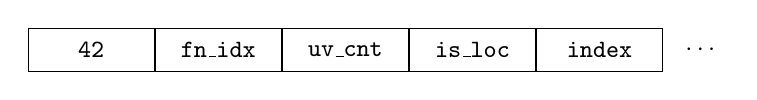
\begin{tikzpicture}[
  byte/.style={draw, minimum width=1.6cm, minimum height=0.55cm, font=\small\ttfamily},
]
\node[byte] (op) at (0,0) {42};
\node[byte, right=0pt of op] (idx) {fn\_idx};
\node[byte, right=0pt of idx] (cnt) {uv\_cnt};
\node[byte, right=0pt of cnt] (l1) {is\_loc};
\node[byte, right=0pt of l1] (i1) {index};
\node[font=\small] at ($(i1.east)+(0.5,0)$) {$\cdots$};
\end{tikzpicture}
\end{center}

\noindent
The \texttt{fn\_idx} operand indexes into the chunk's constant pool, where
the function's compiled \texttt{Chunk} is stored as a \texttt{VAL\_CLOSURE}
constant.  The \texttt{uv\_cnt} byte gives the number of upvalue descriptors
that follow, each a pair \texttt{[is\_local, index]}.  The wide variant
\opcode{CLOSURE\_16} uses a two-byte big-endian function index.

\subsection{Runtime Representation}

Open upvalues are represented by the \texttt{ObjUpvalue} struct:

\begin{lstlisting}[style=clang,caption={The ObjUpvalue structure.}]
typedef struct ObjUpvalue {
    LatValue *location;      // -> stack slot (open)
    LatValue  closed;        //    or &closed (closed)
    struct ObjUpvalue *next; // linked list
} ObjUpvalue;
\end{lstlisting}

While a variable is still on the stack, \texttt{location} points directly
into the stack slot.  The VM maintains a singly linked list of all open
upvalues, sorted by stack address in descending order.  This ordering
enables efficient insertion and lookup during capture.

\subsection{Capture and Closure}

When executing \opcode{CLOSURE}, the VM processes each upvalue descriptor:

\begin{itemize}
  \item If \texttt{is\_local = 1}: call \texttt{capture\_upvalue()}, which
    walks the open upvalue list to find an existing upvalue pointing at the
    same stack slot.  If found, it is reused (ensuring multiple closures
    share the same upvalue).  Otherwise, a new \texttt{ObjUpvalue} is created
    and inserted into the sorted list.
  \item If \texttt{is\_local = 0}: copy the upvalue pointer from the
    enclosing frame's upvalue array at the given index.
\end{itemize}

When a local variable goes out of scope (\opcode{CLOSE\_UPVALUE}), the VM
calls \texttt{close\_upvalues()}: each open upvalue whose \texttt{location}
is at or above the target stack address is \emph{closed} by deep-cloning the
pointed-to value into \texttt{closed} and redirecting \texttt{location} to
\texttt{\&closed}.  This approach, inspired by Lua's upvalue
design~\cite{ierusalimschy2005implementation} and refined by
Nystrom~\cite{nystrom2021crafting}, ensures that closed-over variables
survive beyond their lexical scope without garbage collector integration.

\subsection{The Storage Hack}

The bytecode VM repurposes existing fields of the \texttt{LatValue} closure
representation to avoid adding VM-specific fields:

\begin{itemize}
  \item \texttt{closure.body} is \texttt{NULL} for compiled functions (the
    tree-walker uses this field for the AST body).
  \item \texttt{closure.native\_fn} stores a \texttt{Chunk*} pointer to the
    compiled function body.
  \item \texttt{closure.captured\_env} is cast to \texttt{ObjUpvalue**},
    storing the array of captured upvalue pointers.
  \item \texttt{region\_id} stores the upvalue count (since compiled
    closures do not participate in region tracking).
\end{itemize}

To distinguish VM-native C functions (registered via
\texttt{vm\_register\_native()}) from compiled closures, a sentinel
value is used:

\begin{lstlisting}[style=clang]
#define VM_NATIVE_MARKER ((struct Expr **)(uintptr_t)0x1)
\end{lstlisting}

\noindent
A closure with \texttt{body == NULL}, \texttt{native\_fn != NULL}, and
\texttt{default\_values == VM\_NATIVE\_MARKER} is a C-native function;
one with \texttt{body == NULL} and \texttt{native\_fn != NULL} but without
the marker is a compiled bytecode closure.

\subsection{Walkthrough: Compilation and Execution}

To illustrate the complete pipeline, consider the following Lattice program
that demonstrates closure capture:

\begin{lstlisting}[caption={A closure capturing a local variable.}]
fn make_counter() {
    flux count = 0
    return fn() {
        count += 1
        return count
    }
}
let c = make_counter()
print(c())  // 1
print(c())  // 2
\end{lstlisting}

\paragraph{Compilation.}
The compiler processes \texttt{make\_counter} by creating a nested
\texttt{Compiler}.  The inner closure references \texttt{count}, which is
a local in the enclosing function.  The compiler:

\begin{enumerate}
  \item Resolves \texttt{count} via \texttt{resolve\_upvalue()}, which finds
    it as local slot~1 in \texttt{make\_counter} and marks it as captured.
  \item Calls \texttt{add\_upvalue()} with \texttt{index=1, is\_local=true}.
  \item Compiles \texttt{count += 1} as: \opcode{GET\_UPVALUE}~0,
    \opcode{LOAD\_INT8}~1, \opcode{ADD}, \opcode{SET\_UPVALUE}~0, \opcode{POP}.
  \item Stores the inner function's chunk as a constant in
    \texttt{make\_counter}'s chunk.
  \item Emits \opcode{CLOSURE}~\texttt{[fn\_idx, 1, 1, 1]} --- one upvalue,
    \texttt{is\_local=1}, \texttt{index=1}.
\end{enumerate}

When \texttt{make\_counter} returns, the compiler emits \opcode{CLOSE\_UPVALUE}
for the captured local \texttt{count} (rather than a plain \opcode{POP}).

\paragraph{Execution.}
At runtime:
\begin{enumerate}
  \item \opcode{CLOSURE} executes: \texttt{capture\_upvalue()} creates an
    \texttt{ObjUpvalue} pointing at \texttt{frame->slots[1]} (where
    \texttt{count} lives), and inserts it into the VM's open upvalue list.
  \item When \texttt{make\_counter} returns, \opcode{CLOSE\_UPVALUE} calls
    \texttt{close\_upvalues()}: the upvalue's \texttt{closed} field receives
    a deep clone of the stack value, and \texttt{location} is redirected
    to \texttt{\&closed}.
  \item Each call to \texttt{c()} accesses \texttt{count} via
    \opcode{GET\_UPVALUE}~0, which dereferences \texttt{location} ---
    now pointing to the heap-allocated \texttt{closed} field.
  \item Successive calls correctly see the incrementing value because
    \opcode{SET\_UPVALUE}~0 writes through the same \texttt{location}
    pointer.
\end{enumerate}

%% ─────────────────────────────────────────────────────────────────────────────
\section{VM Execution Engine}
\label{sec:engine}

\subsection{VM State}

\needspace{20\baselineskip}
The VM maintains the following state:

\begin{lstlisting}[style=clang,caption={VM structure (abridged).}]
typedef struct {
    CallFrame  frames[256];    // call frame stack
    size_t     frame_count;
    LatValue   stack[4096];    // value stack
    LatValue  *stack_top;
    Env       *env;            // global variables
    ObjUpvalue *open_upvalues; // linked list
    ExceptionHandler handlers[64];
    size_t     handler_count;
    VMDeferEntry defers[256];
    size_t     defer_count;
    LatValue   fast_args[16];  // pre-allocated
    BumpArena *ephemeral;      // arena for temps
    LatMap     module_cache;
    // phase system: tracked vars, pressures,
    //   reactions, bonds, seeds ...
} VM;
\end{lstlisting}

\needspace{10\baselineskip}
Each call frame records the chunk being executed, the instruction pointer,
a base pointer into the value stack, and the frame's upvalue array:

\begin{lstlisting}[style=clang]
typedef struct {
    Chunk      *chunk;
    uint8_t    *ip;
    LatValue   *slots;  // frame base on stack
    ObjUpvalue **upvalues;
    size_t      upvalue_count;
} CallFrame;
\end{lstlisting}

\subsection{Dispatch Loop}

The VM's inner loop reads one opcode per iteration and dispatches to the
corresponding handler.  On compilers supporting the GCC/Clang labels-as-values
extension, we use \emph{computed goto} via a dispatch table:

\begin{lstlisting}[style=clang,caption={Dispatch loop (simplified).}]
#define READ_BYTE() (*frame->ip++)
#define READ_U16()  (frame->ip += 2, \
    (uint16_t)((frame->ip[-2] << 8) | frame->ip[-1]))

#ifdef VM_USE_COMPUTED_GOTO
  static void *dispatch_table[] = {
    [OP_CONSTANT] = &&lbl_OP_CONSTANT,
    [OP_NIL]      = &&lbl_OP_NIL,
    // ... all 100 entries
  };
#endif

for (;;) {
    uint8_t op = READ_BYTE();
#ifdef VM_USE_COMPUTED_GOTO
    goto *dispatch_table[op];
#endif
    switch (op) {
#ifdef VM_USE_COMPUTED_GOTO
        lbl_OP_CONSTANT:
#endif
        case OP_CONSTANT: { /* ... */ }
        // ...
    }
}
\end{lstlisting}

Computed goto eliminates the overhead of the switch statement's bounds check
and branch table lookup, replacing it with a single indirect jump per
instruction.  On platforms without the extension, the compiler falls back
to a standard switch.

\subsection{Call Protocol}

The \opcode{CALL} instruction discriminates three callee types:

\paragraph{Native functions.}
If the callee is marked with \texttt{VM\_NATIVE\_MARKER}, the VM pops
arguments into a pre-allocated \texttt{fast\_args[16]} buffer (falling back
to \texttt{malloc} for calls with more than 16 arguments), invokes the
C function pointer, and pushes the return value.  This fast path avoids
allocating a new call frame entirely.

\paragraph{Compiled closures.}
The VM first promotes all ephemeral values in the current frame to prevent
the callee's \opcode{RESET\_EPHEMERAL} from invalidating the caller's
temporaries.  It then pushes a new \texttt{CallFrame} pointing to the
callee's chunk, with the instruction pointer at byte~0 and the stack base
set to the callee's position on the stack (so \texttt{slots[0]} is the
closure itself, followed by arguments in \texttt{slots[1..arity]}).

\paragraph{Callable structs.}
If the callee is a struct value, the VM looks for a field named with
the struct's type (constructor convention) and dispatches accordingly.

\subsection{Exception Handling}

Exception handlers are registered by \opcode{PUSH\_EXCEPTION\_HANDLER}, which
records the current instruction pointer, chunk, call frame index, and stack
top.  When \opcode{THROW} executes:

\begin{enumerate}
  \item The nearest handler is popped from the handler stack.
  \item The call frame stack is unwound to the handler's frame index.
  \item The value stack is restored to the handler's recorded stack top.
  \item The error value is pushed onto the stack.
  \item Execution resumes at the handler's saved IP (the catch block).
\end{enumerate}

Deferred blocks interact correctly: \opcode{DEFER\_RUN} executes all defer
entries registered at or above the current frame before the frame is popped
by \opcode{RETURN}.

\subsection{Iterators}

The \opcode{ITER\_INIT} instruction converts a range or array value into an
internal iterator representation occupying two stack slots (the collection
and a cursor index).  The \opcode{ITER\_NEXT} instruction advances the
cursor, pushes the next element, or jumps to the specified offset when
exhausted.  This design avoids allocating a closure object for
\texttt{for}~loops, unlike the tree-walker which used closure-based iterators.

\subsection{Architecture Overview}

Figure~\ref{fig:vm-arch} illustrates the VM's runtime data structures and
their relationships.

\begin{figure}[H]
\centering
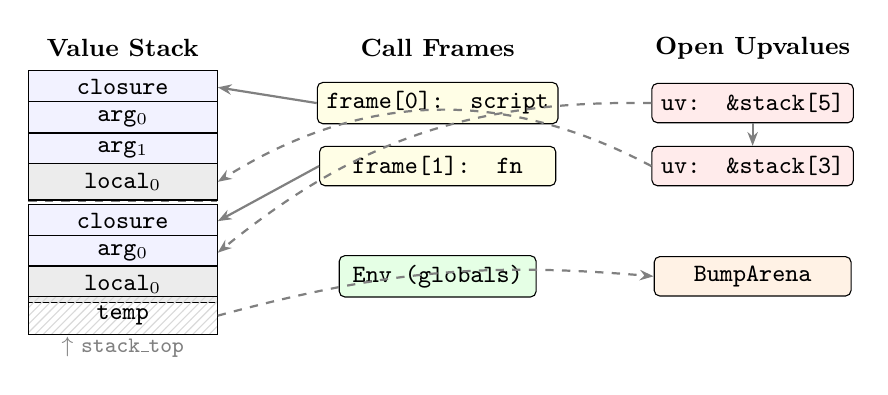
\begin{tikzpicture}[
  box/.style={draw, rounded corners=2pt, minimum width=2cm, minimum height=0.5cm,
              font=\small\ttfamily, fill=white},
  stack/.style={draw, minimum width=2.4cm, minimum height=0.4cm,
                font=\small\ttfamily, fill=blue!5},
  arr/.style={-{Stealth[length=5pt]}, thick},
]
% Value stack
\node[font=\small\bfseries] at (0, 3.2) {Value Stack};
\node[stack] (s0) at (0, 2.7) {closure};
\node[stack] (s1) at (0, 2.3) {arg$_0$};
\node[stack] (s2) at (0, 1.9) {arg$_1$};
\node[stack, fill=gray!15] (s3) at (0, 1.5) {local$_0$};
\draw[dashed, gray] (-1.2, 1.25) -- (1.2, 1.25);
\node[stack] (s4) at (0, 1.0) {closure};
\node[stack] (s5) at (0, 0.6) {arg$_0$};
\node[stack, fill=gray!15] (s6) at (0, 0.2) {local$_0$};
\node[stack, pattern=north east lines, pattern color=gray!30] (s7) at (0, -0.2) {temp};
\node[font=\footnotesize, gray] at (0, -0.6) {$\uparrow$ \texttt{stack\_top}};

% Call frames
\node[font=\small\bfseries] at (4, 3.2) {Call Frames};
\node[box, fill=yellow!10, minimum width=3cm] (f0) at (4, 2.5) {frame[0]: script};
\node[box, fill=yellow!10, minimum width=3cm] (f1) at (4, 1.7) {frame[1]: fn};

\draw[arr, gray] (f0.west) -- (s0.east);
\draw[arr, gray] (f1.west) -- (s4.east);

% Globals
\node[box, fill=green!10, minimum width=2.5cm] (env) at (4, 0.3) {Env (globals)};

% Upvalues
\node[font=\small\bfseries] at (8, 3.2) {Open Upvalues};
\node[box, fill=red!8, minimum width=2.5cm] (uv0) at (8, 2.5) {uv: \&stack[5]};
\node[box, fill=red!8, minimum width=2.5cm] (uv1) at (8, 1.7) {uv: \&stack[3]};
\draw[arr, gray] (uv0.south) -- (uv1.north);
\draw[arr, dashed, gray] (uv0.west) to[bend right=20] (s5.east);
\draw[arr, dashed, gray] (uv1.west) to[bend right=30] (s3.east);

% Ephemeral
\node[box, fill=orange!10, minimum width=2.5cm] (arena) at (8, 0.3) {BumpArena};
\draw[arr, dashed, gray] (s7.east) to[bend left=10] (arena.west);
\end{tikzpicture}
\caption{VM runtime architecture: value stack with frame boundaries, call
frame stack, global environment, open upvalue linked list, and ephemeral
bump arena.}
\label{fig:vm-arch}
\end{figure}

%% ─────────────────────────────────────────────────────────────────────────────
\section{Compiling Concurrency Primitives}
\label{sec:concurrency}

\subsection{The Problem}

Lattice provides structured concurrency through three primitives:
\texttt{scope} (defines a concurrent region), \texttt{spawn} (launches
a lightweight task within a scope), and \texttt{select} (multiplexes over
channels).  In the tree-walking interpreter, these primitives evaluate
sub-expressions by passing AST node pointers to spawned threads.  This
creates a hard dependency: the AST must remain live for the duration of
concurrent execution, and the program cannot be serialized to bytecode alone.

\subsection{Pre-Compiled Sub-Chunks}

The solution is to compile each concurrent body into a standalone
\texttt{Chunk} at compile time.  The compiler provides two helper functions:

\begin{itemize}
  \item \texttt{compile\_sub\_body(stmts, count, line)}: Saves the current
    compiler, creates a fresh \texttt{Compiler} with type \texttt{FUNC\_SCRIPT},
    compiles the statement list, emits \opcode{HALT}, restores the outer
    compiler, and returns the resulting \texttt{Chunk}.
  \item \texttt{compile\_sub\_expr(expr, line)}: Similar, but compiles a
    single expression and emits \opcode{HALT} after it.
\end{itemize}

The resulting chunk is stored in the parent chunk's constant pool as a
\texttt{VAL\_CLOSURE} constant (using the same storage hack: \texttt{body = NULL},
\texttt{native\_fn = Chunk*}).

\subsection{OP\_SCOPE Encoding and Execution}

The \opcode{SCOPE} instruction uses variable-length encoding:

\begin{center}
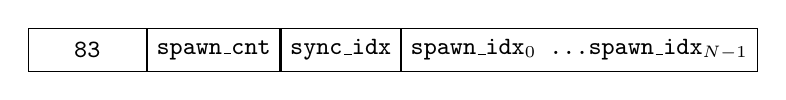
\begin{tikzpicture}[
  byte/.style={draw, minimum width=1.5cm, minimum height=0.55cm, font=\small\ttfamily},
]
\node[byte] (op) at (0,0) {83};
\node[byte, right=0pt of op] (sc) {spawn\_cnt};
\node[byte, right=0pt of sc] (si) {sync\_idx};
\node[byte, right=0pt of si, minimum width=3.5cm] (sp) {spawn\_idx$_0$ \ldots spawn\_idx$_{N-1}$};
\end{tikzpicture}
\end{center}

\noindent
Each index refers to a constant pool entry containing a pre-compiled sub-chunk.
At runtime, \opcode{SCOPE} executes as follows:

\begin{enumerate}
  \item \textbf{Export locals.}  Current frame locals are exported to the
    global environment using the \texttt{local\_names} debug table, so
    sub-chunks (which run as independent scripts) can access them via
    \opcode{GET\_GLOBAL}.
  \item \textbf{Run sync body.}  If \texttt{sync\_idx} is valid (not
    \texttt{0xFF}), the corresponding chunk is executed via a recursive
    \texttt{vm\_run()} call on the same VM.
  \item \textbf{Spawn threads.}  For each spawn index, a child VM is created
    via \texttt{vm\_clone\_for\_thread()} (which clones the environment but
    shares struct metadata), and the spawn body is executed on a new
    \texttt{pthread}.
  \item \textbf{Join.}  All threads are joined; the first error (if any) is
    propagated.
\end{enumerate}

\subsection{OP\_SELECT Encoding and Execution}

The \opcode{SELECT} instruction encodes one record per arm:

\begin{center}
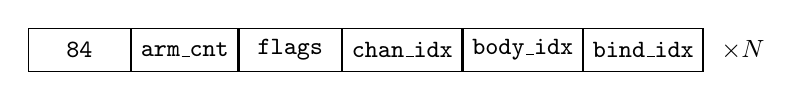
\begin{tikzpicture}[
  byte/.style={draw, minimum width=1.3cm, minimum height=0.55cm, font=\small\ttfamily},
]
\node[byte] (op) at (0,0) {84};
\node[byte, right=0pt of op] (ac) {arm\_cnt};
\node[byte, right=0pt of ac] (fl) {flags};
\node[byte, right=0pt of fl] (ch) {chan\_idx};
\node[byte, right=0pt of ch] (bi) {body\_idx};
\node[byte, right=0pt of bi] (bn) {bind\_idx};
\node[font=\small] at ($(bn.east)+(0.5,0)$) {$\times N$};
\end{tikzpicture}
\end{center}

\noindent
Each arm specifies: flags (send vs.\ receive, default arm), the channel
expression's sub-chunk index, the body sub-chunk index, and a binding name
constant index.  At runtime, the VM evaluates channel expressions, polls
for readiness, executes the winning arm's body with the received value
bound to the specified name, or falls through to a default arm.

\subsection{Local Variable Export}

Because sub-chunks are compiled as \texttt{FUNC\_SCRIPT} without lexical
access to the parent's locals, the VM must explicitly export the parent
frame's live locals into the global environment before running any sub-chunk.
This is accomplished by iterating over all active frames' slots, using the
\texttt{chunk->local\_names} debug table to recover variable names, and
calling \texttt{env\_define()} for each.  A scope is pushed before export
and popped after all sub-chunks complete, ensuring the exported bindings
do not leak.

%% ─────────────────────────────────────────────────────────────────────────────
\section{Bytecode Serialization}
\label{sec:serialization}

\subsection{File Format}

The \texttt{.latc} binary format enables ahead-of-time compilation: a
program can be compiled once and the resulting bytecode distributed without
source.  The format begins with an 8-byte header:

\begin{center}
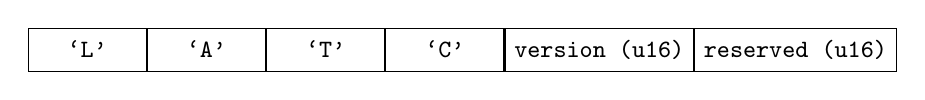
\begin{tikzpicture}[
  byte/.style={draw, minimum width=1.5cm, minimum height=0.55cm, font=\small\ttfamily},
]
\node[byte] (m1) at (0,0) {`L'};
\node[byte, right=0pt of m1] (m2) {`A'};
\node[byte, right=0pt of m2] (m3) {`T'};
\node[byte, right=0pt of m3] (m4) {`C'};
\node[byte, right=0pt of m4, minimum width=2.2cm] (ver) {version (u16)};
\node[byte, right=0pt of ver, minimum width=2.2cm] (res) {reserved (u16)};
\end{tikzpicture}
\end{center}

\noindent
The magic bytes \texttt{"LATC"} identify the format; the 16-bit format
version (currently~1) enables future format evolution; the reserved field
is zero.  All multi-byte integers use little-endian encoding.

\subsection{Chunk Encoding}

Following the header, the top-level chunk is serialized recursively:

\begin{enumerate}
  \item \textbf{Code section:} \texttt{code\_len} (u32) followed by raw
    bytecode bytes.
  \item \textbf{Line section:} \texttt{lines\_len} (u32) followed by
    \texttt{lines\_len} line numbers (u32 each), providing source mapping.
  \item \textbf{Constants section:} \texttt{const\_len} (u32) followed by
    typed constants.
  \item \textbf{Local names section:} \texttt{name\_count} (u32) followed
    by presence flags and strings.
\end{enumerate}

\subsection{Constant Type Tags}

Each constant is prefixed by a one-byte type tag:

\begin{center}
\begin{tabular}{@{}cl@{}}
\toprule
\textbf{Tag} & \textbf{Type and encoding} \\
\midrule
0 & \texttt{Int}: 8-byte signed little-endian \\
1 & \texttt{Float}: 8-byte IEEE~754 double \\
2 & \texttt{Bool}: 1 byte (0 or 1) \\
3 & \texttt{String}: length-prefixed (u32 + bytes) \\
4 & \texttt{Nil}: no payload \\
5 & \texttt{Unit}: no payload \\
6 & \texttt{Closure}: param\_count (u32) + has\_variadic (u8) + recursive chunk \\
\bottomrule
\end{tabular}
\end{center}

The \texttt{Closure} tag enables recursive serialization: a function constant
contains its parameter metadata followed by a complete serialized sub-chunk.
This naturally handles arbitrary nesting depth.

\subsection{Loading and Validation}

The loader (\texttt{chunk\_load()}/\texttt{chunk\_deserialize()}) performs
bounds-checked reading through a \texttt{ByteReader} struct that tracks
position and length.  Validation includes magic byte verification, format
version checking, and graceful error reporting for truncated or malformed
inputs.

\subsection{Example: Byte Layout}

Figure~\ref{fig:latc-layout} shows the byte layout of a minimal
\texttt{.latc} file compiled from \texttt{print(42)}.

\begin{figure}[H]
\centering
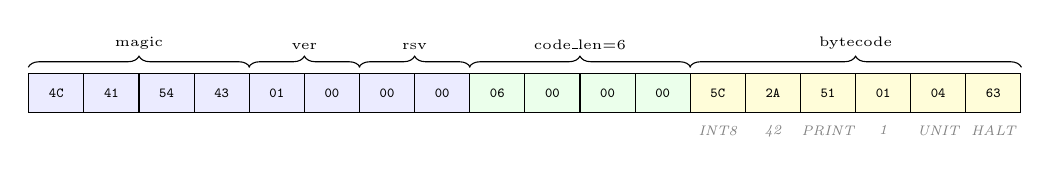
\begin{tikzpicture}[
  byte/.style={draw, minimum width=0.7cm, minimum height=0.5cm, font=\tiny\ttfamily},
  label/.style={font=\tiny\itshape, text=gray},
  brace/.style={decorate, decoration={brace, amplitude=4pt, raise=2pt}},
]
% Header
\foreach \x/\val in {0/4C,1/41,2/54,3/43,4/01,5/00,6/00,7/00} {
  \node[byte, fill=blue!8] (h\x) at (\x*0.7, 0) {\val};
}
\draw[brace] (h0.north west) -- node[above=5pt, font=\tiny] {magic} (h3.north east);
\draw[brace] (h4.north west) -- node[above=5pt, font=\tiny] {ver} (h5.north east);
\draw[brace] (h6.north west) -- node[above=5pt, font=\tiny] {rsv} (h7.north east);

% Code section
\foreach \x/\val in {0/06,1/00,2/00,3/00} {
  \pgfmathtruncatemacro{\xpos}{\x+8}
  \node[byte, fill=green!8] (c\x) at (\xpos*0.7, 0) {\val};
}
\draw[brace] (c0.north west) -- node[above=5pt, font=\tiny] {code\_len=6} (c3.north east);

% Bytecode
\foreach \x/\val in {0/5C,1/2A,2/51,3/01,4/04,5/63} {
  \pgfmathtruncatemacro{\xpos}{\x+12}
  \node[byte, fill=yellow!15] (b\x) at (\xpos*0.7, 0) {\val};
}
\draw[brace] (b0.north west) -- node[above=5pt, font=\tiny] {bytecode} (b5.north east);

% Labels below
\node[label, below=1pt of b0] {INT8};
\node[label, below=1pt of b1] {42};
\node[label, below=1pt of b2] {PRINT};
\node[label, below=1pt of b3] {1};
\node[label, below=1pt of b4] {UNIT};
\node[label, below=1pt of b5] {HALT};
\end{tikzpicture}
\caption{Byte layout of a \texttt{.latc} file for \texttt{print(42)}.
Header bytes shown in blue, code length in green, bytecode in yellow.
The \texttt{LOAD\_INT8}~42 / \texttt{PRINT}~1 / \texttt{UNIT} / \texttt{HALT}
sequence is followed by line number and constant sections (not shown).}
\label{fig:latc-layout}
\end{figure}

\subsection{CLI Integration}

The serialization integrates with the command-line interface:

\begin{itemize}
  \item \texttt{clat compile input.lat [-o out.latc]} compiles source to
    bytecode.
  \item \texttt{clat file.latc} auto-detects the \texttt{.latc} suffix and
    loads pre-compiled bytecode directly, skipping parsing and compilation.
  \item \texttt{clat file.lat} compiles and executes in a single step
    (the default).
\end{itemize}

%% ─────────────────────────────────────────────────────────────────────────────
\section{The Self-Hosted Compiler}
\label{sec:selfhost}

\subsection{Overview}

The file \texttt{compiler/latc.lat} is a self-hosted bytecode compiler
written entirely in Lattice.  At approximately 2,060 lines, it reads
\texttt{.lat} source, produces bytecode, and writes \texttt{.latc} files
using the same binary format as the C implementation.  Usage:

\begin{lstlisting}[language={}]
$ clat compiler/latc.lat input.lat output.latc
$ clat output.latc   # run compiled bytecode
\end{lstlisting}

\subsection{Architecture}

The self-hosted compiler is organized into 12 sections:

\begin{enumerate}
  \item \textbf{Opcode constants} defined as global integers.
  \item \textbf{Compiler state} using parallel global arrays: \texttt{code},
    \texttt{constants}, \texttt{c\_lines}, and \texttt{local\_names} (since
    structs and maps are pass-by-value in Lattice, a struct-based compiler
    state would not propagate mutations through function calls).
  \item \textbf{Lexing} via the built-in \texttt{tokenize()} function, which
    returns an array of token objects.
  \item \textbf{Recursive-descent parser} with functions for each grammar
    production (\texttt{parse\_expression}, \texttt{parse\_statement\_or\_expression}, etc.).
  \item \textbf{Code emission} helpers (\texttt{emit\_byte},
    \texttt{emit\_bytes}, \texttt{emit\_jump}, \texttt{patch\_jump},
    \texttt{emit\_loop}).
  \item \textbf{Scope management} (\texttt{begin\_scope}, \texttt{end\_scope},
    \texttt{add\_local}, \texttt{resolve\_local}, \texttt{resolve\_upvalue}).
  \item \textbf{Function compilation} with a compiler stack using
    \texttt{save\_compiler}/\texttt{restore\_compiler} to handle nested functions.
  \item \textbf{Control flow} (if/else, while, loop, for, break, continue, match).
  \item \textbf{Declarations} (struct, enum, try/catch, defer, import).
  \item \textbf{Top-level entry} (\texttt{compile\_program}).
  \item \textbf{Serializer} writing the \texttt{.latc} binary format to a
    global \texttt{Buffer}.
  \item \textbf{Main} entry point.
\end{enumerate}

\subsection{Language Constraint Workarounds}

Writing a compiler in Lattice required several workarounds for language
semantics that differ from C:

\begin{description}[leftmargin=1.5em]
  \item[Parallel arrays for state.]
    Because structs and maps are pass-by-value, the compiler uses parallel
    global arrays (\texttt{local\_names[]}, \texttt{local\_depths[]},
    \texttt{local\_captured[]}) rather than an array of structs.  Mutations
    to global arrays propagate correctly.

  \item[Global serialization buffer.]
    The \texttt{Buffer} type is also pass-by-value; to accumulate serialized
    bytes across function calls, a global \texttt{ser\_buf} variable is used.

  \item[Compiler stack.]
    Nested function compilation saves and restores compiler state via
    explicit \texttt{save\_compiler()}/\texttt{restore\_compiler()} functions
    that copy all global arrays to local temporaries and back.

  \item[No \texttt{else if}.]
    Lattice requires \texttt{else \{ if \ldots \}} for chained conditionals;
    the \texttt{match} expression is used for dispatch where possible.

  \item[Mandatory type annotations.]
    Function parameters require type annotations (\texttt{fn foo(a: any)}),
    which the self-hosted compiler uses throughout.
\end{description}

\subsection{Coverage}

The self-hosted compiler currently handles: arithmetic and string expressions,
variable declarations and assignments, functions and closures (with upvalue
capture), control flow (if/else, while, loop, for, break, continue, match),
structs, enums, exception handling (try/catch/throw), defer, string
interpolation, and imports.  Not yet implemented: concurrency primitives
(\texttt{scope}/\texttt{spawn}/\texttt{select}) and advanced phase
operations (\texttt{react}, \texttt{bond}, \texttt{seed}).

\subsection{Bootstrapping Path}

The current bootstrapping chain is:

\begin{center}
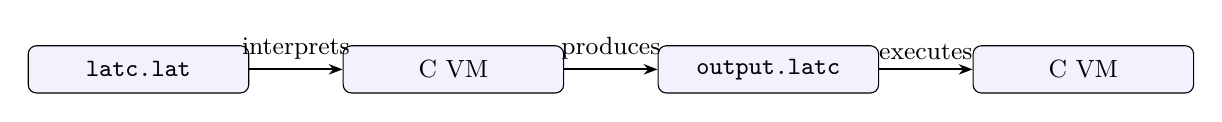
\begin{tikzpicture}[
  box/.style={draw, rounded corners=3pt, minimum width=2.8cm, minimum height=0.6cm,
              font=\small, fill=blue!5},
  arr/.style={-{Stealth[length=5pt]}, thick},
]
\node[box] (src) at (0,0) {\texttt{latc.lat}};
\node[box] (cvm) at (4,0) {C VM};
\node[box] (latc) at (8,0) {\texttt{output.latc}};
\node[box] (run) at (12,0) {C VM};

\draw[arr] (src) -- node[above, font=\small] {interprets} (cvm);
\draw[arr] (cvm) -- node[above, font=\small] {produces} (latc);
\draw[arr] (latc) -- node[above, font=\small] {executes} (run);
\end{tikzpicture}
\end{center}

\noindent
Full self-hosting (where \texttt{latc.lat} compiles itself) requires adding
concurrency support and resolving the remaining feature gaps.

%% ─────────────────────────────────────────────────────────────────────────────
\section{Evaluation}
\label{sec:eval}

\subsection{Test Suite}

The implementation is validated by a comprehensive test suite of
\textbf{815 tests} covering all VM features: arithmetic, closures, upvalues,
phase transitions, exception handling, defer, iterators, data structures,
concurrency, modules, bytecode serialization, and the self-hosted compiler.
All 815 tests pass under both normal compilation and AddressSanitizer
(ASan) builds, confirming the absence of memory errors including
use-after-free, buffer overflows, and memory leaks in the test-exercised
paths.

\subsection{Correctness}

The bytecode VM maintains full parity with the tree-walking interpreter.
Both execution modes share the same test suite and produce identical results:

\begin{lstlisting}[language={}]
$ make test       # bytecode VM (default): 815 passed
$ make test TREE_WALK=1  # tree-walker: 815 passed
\end{lstlisting}

\noindent
This dual-execution model serves as a cross-validation mechanism: any
divergence between the two modes immediately surfaces as a test failure.

\subsection{Feature Completeness}

Table~\ref{tab:parity} summarizes feature coverage across both execution modes.

\begin{table}[H]
\centering
\caption{Feature parity between tree-walker and bytecode VM.}
\label{tab:parity}
\begin{tabular}{@{}lcc@{}}
\toprule
\textbf{Feature} & \textbf{Tree-walker} & \textbf{Bytecode VM} \\
\midrule
Phase system (freeze/thaw/clone/forge)   & \checkmark & \checkmark \\
Closures with upvalues                   & \checkmark & \checkmark \\
Exception handling (try/catch/throw)     & \checkmark & \checkmark \\
Defer blocks                             & \checkmark & \checkmark \\
Pattern matching                         & \checkmark & \checkmark \\
Structs with methods                     & \checkmark & \checkmark \\
Enums with payloads                      & \checkmark & \checkmark \\
Arrays, maps, tuples, sets, buffers      & \checkmark & \checkmark \\
Iterators (for-in, ranges)               & \checkmark & \checkmark \\
Module imports                           & \checkmark & \checkmark \\
Concurrency (scope/spawn/select)         & \checkmark & \checkmark \\
Channels                                 & \checkmark & \checkmark \\
Phase reactions/bonds/seeds              & \checkmark & \checkmark \\
String interpolation                     & \checkmark & \checkmark \\
Contracts (require/ensure)               & \checkmark & \checkmark \\
Variable tracking (history)              & \checkmark & \checkmark \\
Bytecode serialization (.latc)           & ---        & \checkmark \\
Computed goto dispatch                   & ---        & \checkmark \\
Ephemeral bump arena                     & ---        & \checkmark \\
Specialized integer ops                  & ---        & \checkmark \\
\bottomrule
\end{tabular}
\end{table}

\subsection{Test Distribution}

Table~\ref{tab:test-dist} shows the distribution of tests across feature
categories, illustrating the breadth of coverage.

\begin{table}[H]
\centering
\caption{Approximate test distribution by feature category.}
\label{tab:test-dist}
\begin{tabular}{@{}lr@{}}
\toprule
\textbf{Category} & \textbf{Approx.\ tests} \\
\midrule
Core expressions and variables     & 85  \\
Functions and closures             & 75  \\
Control flow (if/while/for/match)  & 70  \\
Data structures (array/map/struct) & 95  \\
Phase system                       & 80  \\
Exception handling and defer       & 45  \\
String operations and interpolation & 50 \\
Concurrency (scope/spawn/select)   & 40  \\
Module imports                     & 30  \\
Enums and pattern matching         & 55  \\
Iterators and ranges               & 35  \\
Bytecode serialization (.latc)     & 25  \\
Integer optimizations              & 20  \\
Contracts (require/ensure)         & 15  \\
Miscellaneous (REPL, tracking, etc.) & 95 \\
\midrule
\textbf{Total}                     & \textbf{815} \\
\bottomrule
\end{tabular}
\end{table}

\subsection{AddressSanitizer Validation}

Running the full test suite under Clang's AddressSanitizer (\texttt{make asan})
enables dynamic detection of:

\begin{itemize}
  \item \textbf{Heap buffer overflows:} Out-of-bounds reads or writes to
    heap-allocated arrays (constant pools, value arrays, etc.).
  \item \textbf{Use-after-free:} Accessing values or chunks that have been
    deallocated---particularly relevant for the upvalue system, where
    closed-over values must outlive their stack slots.
  \item \textbf{Stack buffer overflows:} Overrunning the fixed-size VM
    stacks (4096 value slots, 256 call frames).
  \item \textbf{Memory leaks:} Values or chunks that are allocated but
    never freed (detected via LeakSanitizer, enabled by default with ASan).
\end{itemize}

\noindent
All 815 tests pass under ASan with zero reported errors, providing
confidence in the correctness of memory management throughout the VM,
compiler, and serialization subsystems.

\subsection{Qualitative Assessment}

The bytecode VM provides several structural advantages over the tree-walker:

\begin{itemize}
  \item \textbf{Eliminated AST retention.}  Concurrent execution no longer
    requires keeping AST nodes alive, thanks to pre-compiled sub-chunks.
    This enables bytecode serialization and reduces memory pressure for
    long-running concurrent programs.
  \item \textbf{Reduced dispatch overhead.}  The computed goto dispatch loop
    replaces recursive AST node visits with a flat indirect-jump table,
    eliminating per-node function call overhead and improving branch
    prediction behavior.
  \item \textbf{Serialization.}  The \texttt{.latc} format enables
    compile-once-run-anywhere workflows and eliminates parse/compile time
    on subsequent runs.
  \item \textbf{Foundation for optimization.}  The bytecode representation
    provides a natural target for future optimizations including type
    specialization, register allocation, and JIT compilation.
\end{itemize}

%% ─────────────────────────────────────────────────────────────────────────────
\section{Related Work}
\label{sec:related}

\paragraph{Lua 5.}
Ierusalimschy et al.~\cite{ierusalimschy2005implementation} describe Lua's
register-based bytecode VM, which was a direct inspiration for Lattice's
upvalue design.  Lua's \texttt{UpVal} structure (with open/closed states
and a linked list of open upvalues sorted by stack level) is closely mirrored
by Lattice's \texttt{ObjUpvalue}.  The key difference is that Lattice uses
a stack-based VM rather than a register-based one, accepting slightly larger
bytecode in exchange for simpler code generation and natural expression
evaluation.

\paragraph{CPython.}
CPython~\cite{cpython} uses a stack-based bytecode interpreter with
\texttt{LOAD\_FAST}/\texttt{STORE\_FAST} for locals, a constant pool approach
similar to Lattice's, and a \texttt{.pyc} serialization format.  Lattice
adds the phase system and first-class concurrency primitives as bytecode-level
concepts, which CPython handles at the library level.

\paragraph{Crafting Interpreters.}
Nystrom's \textit{Crafting Interpreters}~\cite{nystrom2021crafting} provides
the pedagogical foundation for the upvalue closure mechanism (open-to-closed
transition via linked list) that Lattice adopts.  Lattice extends this with
phase-aware value semantics: closing an upvalue performs a deep clone rather
than a pointer copy, preserving phase tag integrity.

\paragraph{Ruby YARV.}
The YARV (Yet Another Ruby VM) project~\cite{sasada2005yarv} replaced Ruby's
tree-walking interpreter with a stack-based bytecode VM, motivated by the
same performance concerns that drove Lattice's transition.  YARV uses catch
tables for exception handling; Lattice uses an explicit handler stack, which
simplifies interaction with the defer mechanism.

\paragraph{V8 Ignition.}
The V8 JavaScript engine's Ignition interpreter~\cite{v8ignition} compiles
JavaScript to a register-based bytecode that feeds into the TurboFan
optimizing compiler.  Lattice's bytecode similarly provides a foundation
for future JIT compilation, though the current implementation is
interpreter-only.

\paragraph{Erlang BEAM.}
The BEAM virtual machine~\cite{beam} compiles Erlang to bytecode with
first-class support for lightweight processes and message passing.
Lattice's \opcode{SCOPE} and \opcode{SELECT} instructions serve an
analogous role for structured concurrency.

\paragraph{WebAssembly.}
WebAssembly~\cite{haas2017wasm} uses a stack-based bytecode with a
typed section-based binary format.  Lattice's \texttt{.latc} format shares
the constant-pool-plus-typed-sections approach, though at a higher level
of abstraction (dynamically typed values rather than low-level types).

%% ─────────────────────────────────────────────────────────────────────────────
\section{Conclusion}
\label{sec:conclusion}

We have presented a bytecode virtual machine for the Lattice programming
language that achieves full feature parity with the original tree-walking
interpreter across all language features, including the phase system,
structured concurrency, exception handling, and modules.

The key insight enabling the transition is that concurrency primitives can
be \emph{pre-compiled} into standalone sub-chunks at compile time, stored
in the constant pool, and executed at runtime without any AST dependency.
This eliminates the primary obstacle to bytecode compilation in a language
with first-class structured concurrency.

The 100-opcode instruction set balances generality with targeted
optimizations: wide constant variants handle large programs, specialized
integer operations accelerate common loop patterns, and the ephemeral
bump arena reclaims string temporaries at statement boundaries.  The
\texttt{.latc} serialization format enables ahead-of-time compilation,
and the self-hosted compiler demonstrates that Lattice is expressive
enough to implement its own toolchain.

Future work includes register allocation to reduce stack traffic,
type-specialized dispatch paths guided by runtime profiling,
tail call optimization for recursive patterns, constant pool deduplication
across compilation units, and ultimately JIT compilation targeting the
bytecode as an intermediate representation.

%% ─────────────────────────────────────────────────────────────────────────────
\begin{thebibliography}{99}

\bibitem{jokela2026lattice}
A.~Jokela,
``The Lattice phase system: First-class immutability with dual-heap memory management,''
Technical report, 2026.

\bibitem{jokela2026arena}
A.~Jokela,
``Ephemeral bump arena for a bytecode virtual machine: Design and memory safety proof,''
Technical report, 2026.

\bibitem{ierusalimschy2005implementation}
R.~Ierusalimschy, L.~H. de~Figueiredo, and W.~Celes,
``The implementation of Lua~5.0,''
\textit{Journal of Universal Computer Science}, vol.~11, no.~7, pp.~1159--1176, 2005.

\bibitem{nystrom2021crafting}
R.~Nystrom,
\textit{Crafting Interpreters}.
Genever Benning, 2021.

\bibitem{cpython}
Python Software Foundation,
``CPython: The reference implementation of Python,''
\url{https://github.com/python/cpython}.

\bibitem{sasada2005yarv}
K.~Sasada,
``YARV: Yet another RubyVM,''
In \textit{Companion to the 20th Annual ACM SIGPLAN Conference on Object-Oriented Programming, Systems, Languages, and Applications}, pp.~158--159, 2005.

\bibitem{v8ignition}
R.~Hindley,
``Firing up the Ignition interpreter,''
V8 Blog, 2016.
\url{https://v8.dev/blog/ignition-interpreter}.

\bibitem{beam}
J.~Armstrong,
``A history of Erlang,''
In \textit{Proceedings of the Third ACM SIGPLAN Conference on History of Programming Languages}, pp.~6-1--6-26, 2007.

\bibitem{haas2017wasm}
A.~Haas, A.~Rossberg, D.~L. Schuff, B.~L. Titzer, M.~Holman, D.~Gohman,
L.~Wagner, A.~Zakai, and J.~Bastien,
``Bringing the web up to speed with WebAssembly,''
In \textit{Proceedings of the 38th ACM SIGPLAN Conference on Programming Language Design and Implementation}, pp.~185--200, 2017.

\bibitem{ierusalimschy2003evolution}
R.~Ierusalimschy, L.~H. de~Figueiredo, and W.~Celes,
``The evolution of Lua,''
In \textit{Proceedings of the Third ACM SIGPLAN Conference on History of Programming Languages}, pp.~2-1--2-26, 2007.

\bibitem{lattice2026semantics}
A.~Jokela,
``Formal semantics of the Lattice phase system,''
Technical report, 2026.

\end{thebibliography}

\end{document}
